\section{An exocentric vision system for Morduc}
\label{sec:concr}
This section will show how to use \textsf{REAR} to implement a 
concrete exocentric vision system, specifically designed for 
Morduc.
%

%
As section \ref{sec:rear} explains, in order to get things 
done, all we need to write is:
\begin{itemize}
\item a concrete subclass of \texttt{Robot}
\item an implementation of the \texttt{IDataLogic} interface
\item an implementation of the \texttt{IImageSelector} interface
\end{itemize}
%
The class diagram of the complete system is reported in figure 
\ref{fig:class_diagram_complete}. 
%
As it's easy to notice, it features two implementations 
of the \texttt{IImageSelector} interface: \texttt{SpacialMetricCalc} 
and \texttt{SweepMetricCalc}. The former is a variant 
of the image selection method 2 reported in \cite{sugimoto} and 
whose possible implementation is showed in section 
\ref{sub:iimageselector}.
%

%
\begin{figure}[!h]
  \begin{center}
    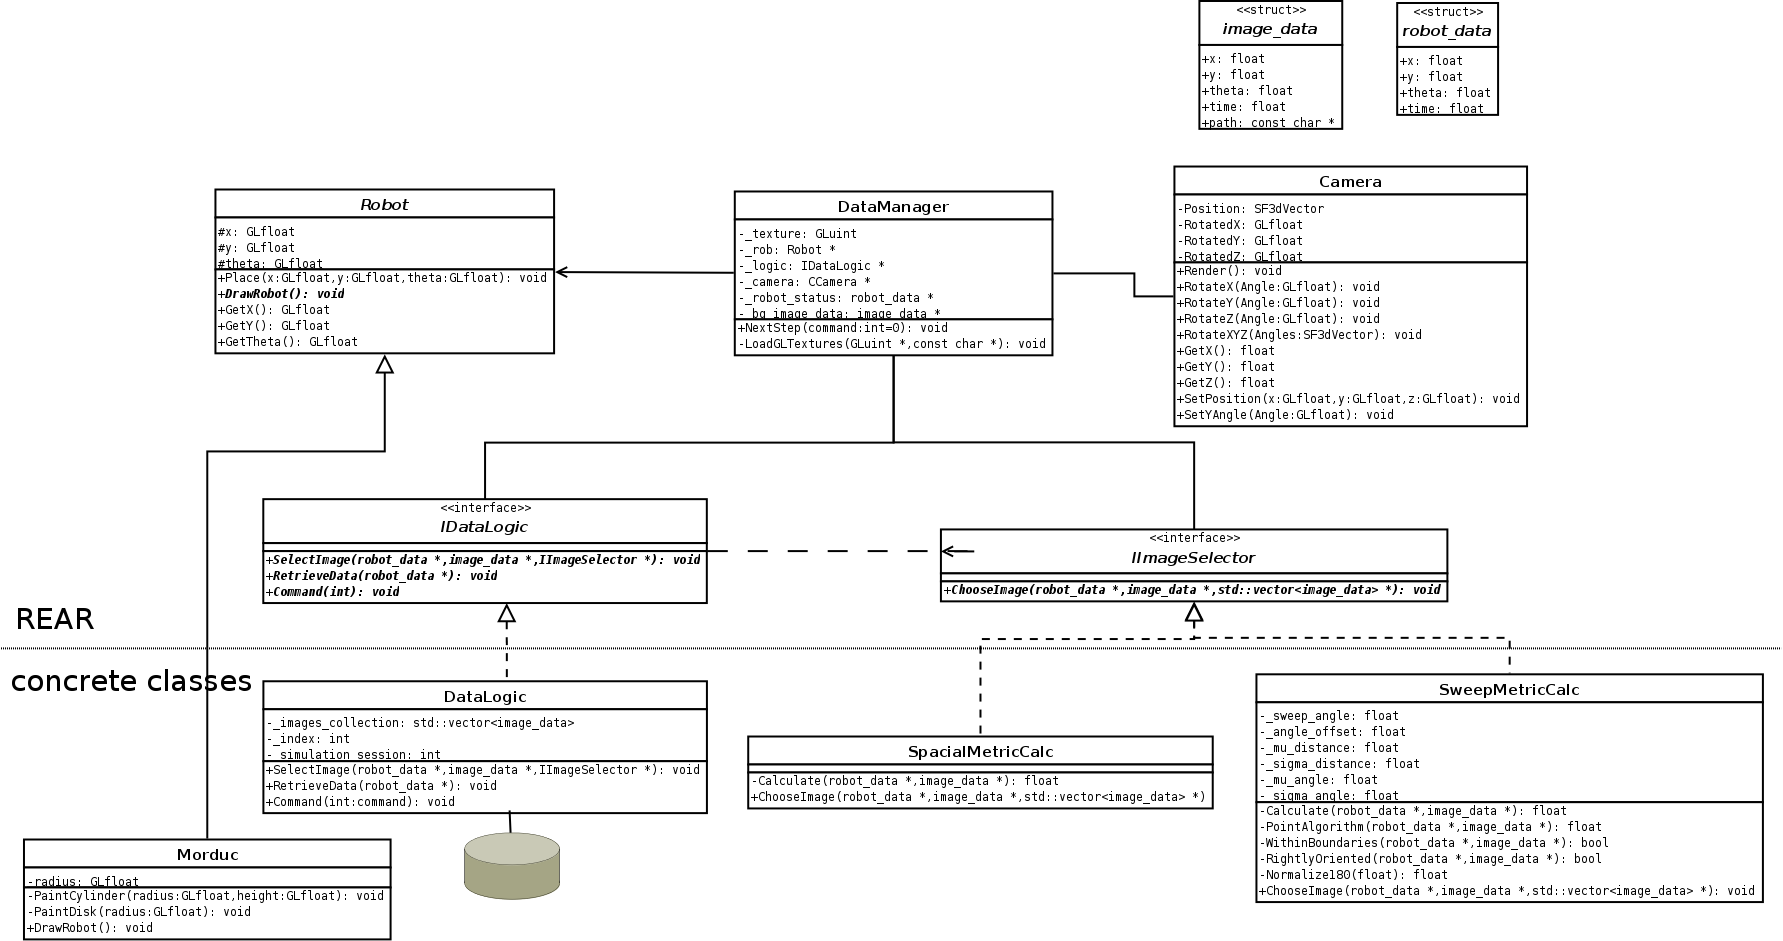
\includegraphics[width=400pt]{img/class_diagram.png} 
    \caption{Class diagram of the whole system}
    \label{fig:class_diagram_complete}
  \end{center}
\end{figure}
%

The latter, instead, encapsulates a brand new selection algorithm. 
It will be widely discussed later in section 
\ref{subsec:sweep_metric_algorithm}.


\subsection{The Morduc Class}
\label{subsec:morducclass}

The \texttt{Morduc} class publicly inherits from \texttt{Robot} 
and, hence, implements the \texttt{DrawRobot()} method:
%
\begin{lstlisting}[caption={\texttt{Morduc} class declaration}, label={code:morducclass}, frame=trBL]
class Morduc : public Robot
{
 private:
  GLfloat radius;
  void PaintCylinder(GLfloat radius,GLfloat height);
  void PaintDisk(GLfloat radius);

 public:
  Morduc(float radius = 4.0f);
  void DrawRobot();
};
\end{lstlisting}
%
Such a method, reported in listing \ref{code:drawrobot}, contains the 
procedure to actually draw the OpenGL model representing Murdoc 
(in reality, Murdoc looks like a stack of three disks linked 
by thin cylinders - see figure \ref{fig:3morduc_opengl}).
%
\begin{lstlisting}[caption={\texttt{Morduc::DrawRobot()} function}, label={code:drawrobot}, frame=trBL]
void Morduc::DrawRobot()
{
  GLfloat reflectance_black[] = { 0.2f, 0.2f, 0.2f};
  GLfloat reflectance_white[] = { 0.8f, 0.8f, 0.8f};
  
  glMatrixMode(GL_MODELVIEW);  
  glPushMatrix();

  // set robot reflectance (it is black)
  glMaterialfv(GL_FRONT_AND_BACK, GL_AMBIENT, 
               reflectance_black);

  // set robot position
  glTranslatef(this -> x, 0.0f, this -> y);

  glRotatef(this -> theta, 0.0f, 1.0f, 0.0f);
  
  // translate on z axis
  // not to make the robot wipe the floor
  glTranslatef(0.0f,0.08f,0.0f);

  glScalef(radius, radius, radius);
  
  // draw robot
  PaintCylinder(1.0f, 0.1);
  PaintDisk(-1.0f);
  glTranslatef(0.0f, 0.1f, 0.0f);
  PaintDisk(1.0f);
  
  glTranslatef(0.0f, 0.6f, 0.0f);

  PaintCylinder(1.0f, 0.1f);
  PaintDisk(-1.0f);
  glTranslatef(0.0f, 0.1f, 0.0f);
  PaintDisk(1.0f);

  glTranslatef(0.8f, 0.0f, 0.0f);
  glColor3f(0.5f, 0.5f, 0.5f);
  PaintCylinder(0.2f, 0.3f);
  glTranslatef(0.0f, 0.3f, 0.0f);
  PaintDisk(0.2f);

  glTranslatef(0,0.401,0);
  glMaterialfv(GL_FRONT_AND_BACK, GL_AMBIENT, 
               reflectance_white);
  PaintDisk(0.1f);
  glTranslatef(0,-0.701,0);
  glMaterialfv(GL_FRONT_AND_BACK, GL_AMBIENT, 
               reflectance_black);

  glTranslatef(-0.8f, 0.0f, 0.0f);
  glColor3f(0.1f, 0.1f, 0.1f);
  glTranslatef(0.0f ,0.6f, 0.0f);
  PaintCylinder(1.0f, 0.1f);
  PaintDisk(-1.0f);
  glTranslatef(0.0f, 0.1f, 0.0f); 
  PaintDisk(1.0f);

  glTranslatef(0.0f, -1.5f, 0.0f);
  glTranslatef(0.0f, 0.0f, 0.8f);
  PaintCylinder(0.1f, 1.5f);
  glTranslatef(0.0f, 0.0f, -1.60f);
  PaintCylinder(0.1f, 1.5f);
  glTranslatef(-0.8f, 0.0f, 0.8f);

  PaintCylinder(0.1f, 1.5f);
  glTranslatef(0.8f, 0.0f, 0.0f);

  glScalef(1/radius, 1/radius, 1/radius);

  glPopMatrix();
}
\end{lstlisting}
%
Notice how such a function implements the skeleton 
presented in listing \ref{code:drawrobot_skeleton}.
%

%
As you have surely noticed, \texttt{Morduc} contains also 
some private attributes, precisely two methods - 
\texttt{PaintCylinder()} and \texttt{PaintDisk()} - and 
a float field - \texttt{radius}.
%
The two methods are just \textit{helper functions}, that is, 
functions that contains a procedure to draw, respectively,  
a \textit{disk} and a \textit{cylinder}.
%
\texttt{radius}, instead, stores the value of the radius 
for the of the cylinders which make up the robot.
%
\begin{figure}[!h]
  \begin{center}
    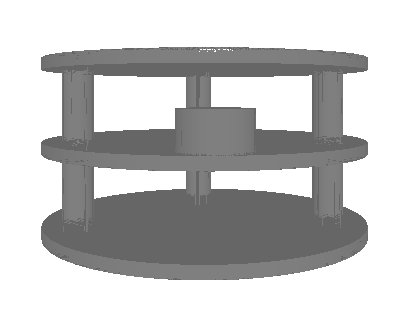
\includegraphics[width=200pt]{img/3morduc_opengl.png}
    \caption{Three dimensional model of Morduc}
    \label{fig:3morduc_opengl}
  \end{center}
\end{figure}
%
After some calibration, the default \texttt{radius} value 
has been set to 4.0.
%

%
\subsection{The DataLogic Class}
\label{sub:datalogic}
For the reasons explained in section \ref{sec:simulator}, 
we used a Morduc simulator in order to generate and record 
test data to use during \textit{offline} tests.
%
For every simulation session, such data consist of:
%
\begin{itemize}
  \item a set of captured images, encoded in the png format
  \item a log file reporting sampled odometry data
\end{itemize}
%
The format of the log file is the one described in section 
\ref{sec:simulator}.
%

%
The concrete \texttt{DataLogic} class will, then, provide 
robot's odometry data and snapshots simply by reading 
those files.
%
Let us have a look at its declaration:
%
\begin{lstlisting}[caption={\texttt{DataLogic} declaration}, label={code:datalogic}, frame=trBL]
class DataLogic : public IDataLogic
{
 private:
  std::vector<image_data> _images_collection;
  int _index;
  int _simulation_session;
  
 public:
  DataLogic(int);
  ~DataLogic();
  void Command(int);
  void RetrieveData(robot_data *);
  void SelectImage(robot_data *, image_data *,
		   IImageSelector *);
};
\end{lstlisting}
%
Upon instantiation, \texttt{DataLogic} objects needs to be 
configured with a session identifier, to be passed to 
the constructor. 
%

%
In order for the \texttt{DataLogic} objects to find them, 
log data must be stored within the relative path 
\texttt{../log}, with respect to the actual execution path.
%
Such a directory must contain a single subdirectory for every 
logged session, named \texttt{log\_$\langle$number of session$\rangle$}. 
%

%
Let us now have a look at how \texttt{DataLogic} implements 
\texttt{IDataLogic} methods:
%
\begin{lstlisting}[caption={\texttt{DataLogic::Command() method}}, label={code:command_method}, frame=trBL]
void DataLogic::Command(int command) 
{

  // sends the command to the robot

  // in our case, just 
  // increase index to point the next line of the file
  _index++;
}
\end{lstlisting}
%
The \texttt{Command()} method is pretty simple in this 
implementation. Since \texttt{DataLogic} has been designed 
for offline testing, there's no actual command to send to the robot.
%
For this reason \texttt{Command()} will not take into account
the received command, the only thing that it does is 
incrementing the private attribute \texttt{\_index}, which 
will be used by \texttt{RetrieveData()} to select which line 
of the log file is to read next.
%
\begin{lstlisting}[caption={\texttt{DataLogic::RetrieveData()} method}, label={code:retrievedata_method}, frame=trBL]
void DataLogic::RetrieveData(robot_data * data)
{
  // pointer to text file containing data
  FILE * position_data;
  char line[50];
  
  std::string * line_read;
  std::string line_values[4];
  std::string position_data_name;
  std::ostringstream o;
  
  int time;
  int line_number = _index;

  // grabbed image metadata
  image_data grabbed_frame_data;
  
  o << "../log/log_" 
    << _simulation_session 
    << "/data_" 
    << _simulation_session << ".txt";

  position_data_name = o.str();

  position_data = fopen(position_data_name.c_str(), "rt");

  while(fgets(line, 50, position_data) &&
	line_number > 1)
    {
      line_number--;
    }

  line_read = new std::string(line);

  std::string buf;
  std::stringstream ss(*line_read);

  // Create vector to hold our words
  std::vector<std::string> tokens;
  
  // put token in vector element
  while (ss >> buf)
    tokens.push_back(buf);

  data->x = atof ( tokens[0].c_str() );
  data->y = atof( tokens[1].c_str() );
  data->theta = TO_DEGREES(- atof ( tokens[2].c_str() ));
  data->time = atof ( tokens[3].c_str() );

  time = (int) data->time;

  // clear the stream and 
  // add a new value to it
  o.str("");
  o.clear();
  o << "../log/log_" 
    << _simulation_session 
    << "/screenshot_" 
    << _simulation_session 
    << "_" << time << ".png";

  // fill grabbed frame metadata
  grabbed_frame_data.x = data->x;
  grabbed_frame_data.y = data->y;
  grabbed_frame_data.theta = data->theta;
  grabbed_frame_data.time = data->time;

  strcpy(grabbed_frame_data.path, o.str().c_str());

  // store the collected metadata 
  // if it's not already stored
  for (std::vector<image_data>::iterator it =
	 _images_collection.begin();
       it != _images_collection.end();
       it++)
    {
      if ( (*it).time == grabbed_frame_data.time )
	{

	  return;
	}
    }

  _images_collection.push_back(grabbed_frame_data);
  return;
}
\end{lstlisting}
%
What the \texttt{RetrieveData()} do is just read the line from the log 
file identified by the \texttt{\_index} private attribute of the class.
Once read, the line is \textit{parsed} and the odometry data contained 
in it is used to fill the \texttt{robot\_data} passed as argument, in 
order to return the \textit{current} robot position.
%
Behind the curtain, \texttt{RetrieveData()} also creates a new 
\texttt{image\_data} structure, fills it with the data just 
gathered and then adds it to the \texttt{\_image\_collection} 
private attribute.
%
This way, every time a new line of the file is read, and, hence, 
every time a new captured image is available, the \texttt{DataLogic} 
is made able to keep track of it using its metadata, without actually 
loading the image - since it would be useless and time-consuming.
%
\begin{lstlisting}[caption={\texttt{DataLogic::SelectImage()} method}, label={code:selectimage_method}, frame=trBL]
void DataLogic::SelectImage(robot_data * robot_status,
                            image_data * bg_image_data,
			    IImageSelector * selector)
{

  // since our data are already stored with vector,
  // we simply pass its reference
  selector -> ChooseImage(robot_status, 
                          bg_image_data, 
                          & _images_collection);
}
\end{lstlisting}
%
Finally, \texttt{SelectImage()} calls the \texttt{ChooseImage} method 
on an object of type \texttt{IImageSelector}, and passes it, as last 
parameter, a reference to its internal \texttt{\_images\_collection}, 
so that the selector can actually select the image to set as 
background.
%
%
%% \texttt{ChooseImage} takes a pointer to the actual robot status and an
%% \texttt{image\_data} pointer used to return the chosen image, the main difference lies in the third (and last)
%% parameter. The concrete \texttt{ChooseImage} requests an \texttt{std::vector} object with all the image stored,
%% whereas a generic \texttt{IDataLogic} implementation can use a different type of set. In this case, the
%% \texttt{ChooseImage} method must convert the generic set containing \texttt{image\_data} in to an \texttt{std::vector},
%% before calling the \texttt{ChooseImage()} method. Finally, the retrieved image will be then returned.
%
\subsection{Image selection algorithms}
\label{sub:metrics}
As already said, there exists many image selection algorithms. 
Three of them are presented in \cite{sugimoto} and, according 
to the results presented, two proved to be unsatisfactory for 
they do not produced results that could effectively improve 
the quality of the operator-robot interaction in situations 
in which the robot moves along comples trajectories.
%
A third one is told to be better but, according to us, it has 
been described poorly and, furthermore, no actual implementation 
of it is given.
%

%
We, then started an investigation on image selection algorithms.
The rest of this chapter will present the theoretical results 
of our investigations: specifically, it will introduce 
two algorithms, which have been implemented by means of 
the definition of two subclasses of the 
\texttt{IImageSelector} interface.
%

%
Both classes use a \texttt{Calculate} method to assign a 
\textit{score}. Such a score is computed according to 
a specific \textit{metric}, that is, a function that, 
given a pair $<$\texttt{robot\_data, image\_data}$>$, 
returns a number. 
%
The \texttt{robot\_data} identifies the robot current position, 
while the \texttt{image\_data} contains the position 
in which the image we want to calculate the score of, 
was taken.
%

%
In both cases, after assigning a score to every collected image, 
the one with the lower score will be returned 
(or better, assigned to the \texttt{image\_data} pointer 
passed to \texttt{IImageSelector::ChooseImage} method).
%

%
This way, it is possible to find which of the snapshots is 
the \textit{closest} (according to the chosen metric) to 
the current robot position.
%
\subsubsection{The spacial metric algorithm}
\label{subsec:spacial_metric_algorithm}
The spacial metric algorithm is a slightly different variant 
of the selection method 2 presented in \cite{sugimoto}.
%
The \texttt{SpacialMetricCalc} class, which encapsulates 
the algorithm, makes use of the Euclidean metric, that is,
its \texttt{Calculate} method returns a value that 
depends from the spacial distance between the current 
robot position and the position in which the snapshot 
was taken.
%

%
Once all spacial distances have been calculated, such values 
are passed as input to the \textit{triangle} function 
showed in picture \ref{fig:spacial_metric_func}.
%
\begin{figure}[!h]
  \begin{center}
    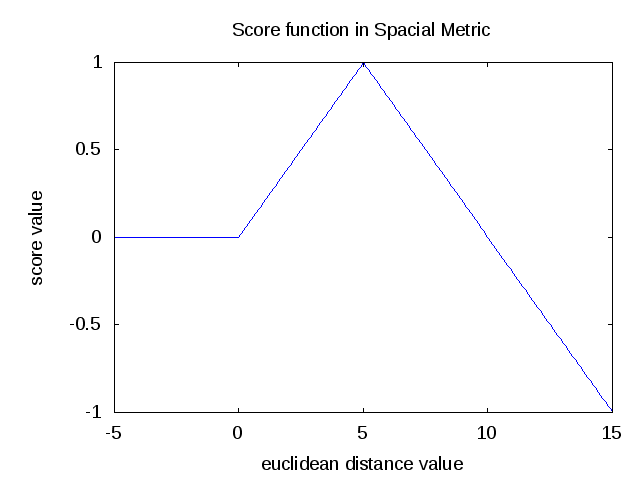
\includegraphics[width=400pt]{img/spacialMetricFunc.png} 
    \caption{Spacial Metric Function}
    \label{fig:spacial_metric_func}
  \end{center}
\end{figure}
%
Since the \texttt{ChooseImage} method will select the image with 
the minimum score, it's easy to figure out that 
images that has been taken when camera was around 
5 spacial units distant from the current robot position
are most likely to bet chosen.
%

%
The motivation lying the algorithm is the following: 
if the euclidean distance of the snapshots from the current 
robot position is around zero, using such images as background 
will result in displaying only a part of the 3D model of the robot.
%
If, instead, such a distance is very high, the model will be drawn 
very far from the camera's (and user's) point-of-view.
%
There, hence, exists, an \textit{optimal distance} that allows 
to draw the robot entirely, but not too far from the camera's 
point-of-view. 
%

%
On the one hand, this algorithm is very simple to implement.
%
On the other hand, it does not care about image orientation. 
%
It could, for instance, choose an image that does not include 
the robot from its point of view. 
%
This limit makes the algorithm good only for situations 
in which the robot moves along straight trajectories.
%
The \textit{Sweep Metric Algorithm}, presented section
\ref{subsec:sweep_metric_algorithm}, will try to go beyond 
this limit.
%

%
\subsubsection{The SpacialMetricCalc class}
The \texttt{SpacialMetricCalc} class encapsulates the 
algorithm presented in the previous section.
%
The value of the \textit{optimal} distance is hardcoded in the
\texttt{Calculate} function:
%
\begin{lstlisting}[caption={\texttt{SweepMetricCalc} class declaration}, label={code:sweepmetriccalc}, frame=trBL]
float SpacialMetricCalc::
          Calculate(robot_data * robot_status, 
                    image_data * bg_image_data) {

  float distance;
  float score;
  float optimal_distance = 20;

  distance = 
    sqrt( pow((robot_status -> x ) - 
              (bg_image_data -> x), 2) +
	  pow((robot_status -> y ) - 
              (bg_image_data -> y), 2) );

  if ( distance <= optimal_distance )
    score = distance / optimal_distance;
 else
    score = - ( distance - 2 * optimal_distance) /
            optimal_distance;

  return (- score);
}
\end{lstlisting}
%
It is not a good solution since, every time one wants to change 
such a values should recompile the code. 
%
On the other hand, this is just a prototype of an algorithm we 
abandoned almost immediately. That is why we did not make any 
code improvement.
%

%
\subsubsection{The sweep metric algorithm}
\label{subsec:sweep_metric_algorithm}
%
The  \textit{Sweep Metric Algorithm}, encapsulated into the 
\texttt{SweepMetricCalc} class, aims at being a more 
complete and flexible image selection algorithm than the one 
we analyzed in the previous section.
%
Let us assume to have  mobile robot moving on a plan, 
taking snapshots from its egocentric-mounted camera.
%
Such a situation is represented in figure 
\ref{fig:half_plan_finding}:
%
\begin{figure}[!h]
  \begin{center}
    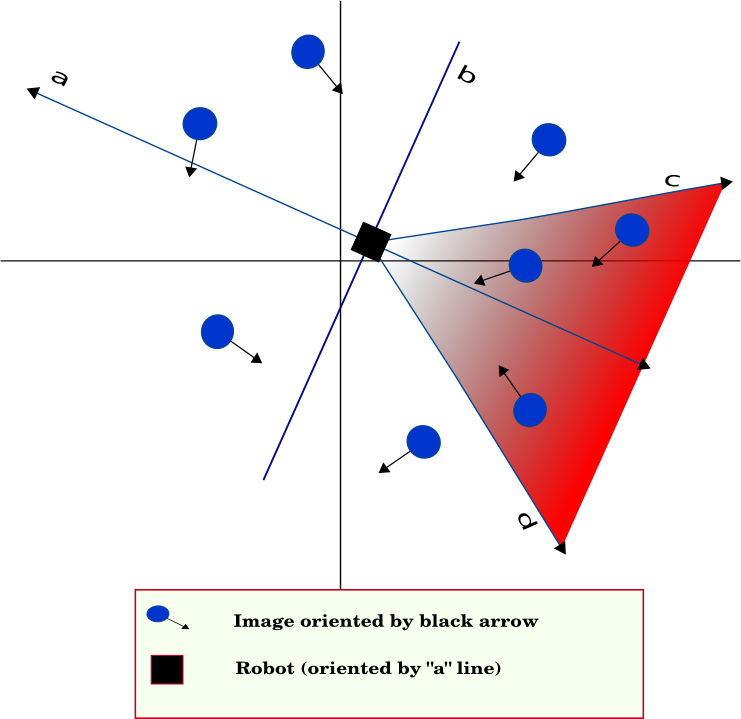
\includegraphics[width=400pt]{img/half_plan_finding.png} 
    \caption{Sweep Angle Algorithm}
    \label{fig:half_plan_finding}
  \end{center}
\end{figure}
%
the black square represents the robot, with its orientation 
indicated by the arrow "a", starting from the square.
%

%
The several blue circles represent instead the previous 
taken images. The orientation of each image - i.e. the 
orientation of the robot when they were taken - 
is shown by an arrow starting from each circle.
%

%
We will refer to the line normal to the half line "a" as "b". 
By rotating clockwise and counterclockwise the "a" line in 
the robot centre with a predefined angle (named "sweep angle")
we will obtain the "c" and "d" lines. These define a new 
portion of the plane (colored with fading red), namely the 
\textit{sweep area}.
%

%
Since we would like to see the robot from its rear, 
all images taken within this area will be taken into account
when selecting the image to set as background.
The other ones will be discarded.
%

%
Then, we have to discard all the images with an orientation 
angle that differs too much from the robot current orientation angle. 
If the difference between the two angles is greater than a specified 
threshold, the image would make the robot being not included 
within the viewing frustum.
%
For instance, if we choose an image whose difference angle with 
the robot current orientation is 180 degrees, it means that robot and 
the camera will be oriented in opposite ways, 
therefore the camera will not see the robot.
%

%
To recognize all discarded images, the \texttt{Calculate} method 
assigns them -2 as score.
%

%
The score of all the remaining image is computed as sum 
of two factors:
%
the first takes into account the image angle orientation: 
the more the image orientation angle is close to the 
robot orientation angle, the more the score is high.
%
\begin{figure}[!h]
  \begin{center}
    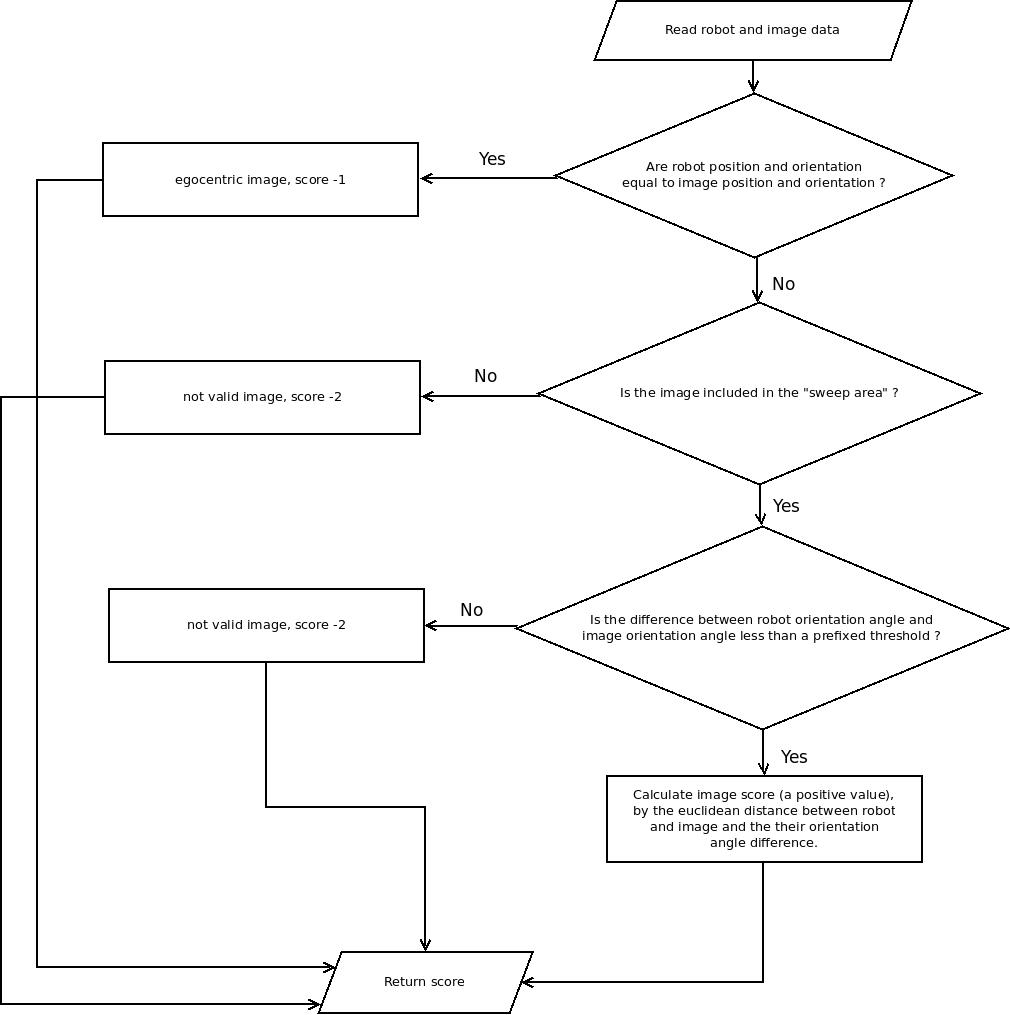
\includegraphics[width=400pt]{img/sweep_angle_diagram.jpeg} 
    \caption{Sweep angle diagram}
    \label{fig:sweep_angle_diagram}
  \end{center}
\end{figure}
%
To compute such a factor, a Gaussian function, centered
in zero, is used. The return value will be therefore 
always a positive number.
%
The use of a Gaussian function allows to obtain different 
values even for two very close angle difference, 
regardless of its variance. 
Moreover, since Gaussian is a surjective function, 
it is defined for all real numbers.
%
This way, images with a little orientation difference with 
the robot current heading will be assigned a higher value.
%

%
The second factor is computed taking into account the Euclidean 
distance between the position in which the image was taken 
and the robot current position. 
%
The approach followed here is the same of the \textit{spacial 
metric algorithm} presented in the previous section: 
given an \textit{optimal} distance, the more the image position 
is close to such a distance, the more the score assigned 
to it will be high.
%
This time, instead of using a \textit{triangle} function, 
we will use a Gaussian function, with a given variance and 
whose centre will be the optimal distance.
%

%
If the image position and orientation coincide with robot position 
and orientation - i.e. the Euclidean distance between the image and 
the robot is zero, the image represents the egocentric vision. 
The score coupled with the egocentric vision will 
always be -1.
%

%
Finally, all computer scores are multiplied by -1 and 
the image with the littlest score is returned.
%

%
If the sweep area does not contain any valid image, all images will
have 2 as score. In such a situation, since the \texttt{ChooseImage} 
search the image with the lowest score, the egocentric image 
will be chosen.
%
\paragraph{The WithinBoundaries algorithm}
\label{par:withinboundaries}
%
Checking if an image is included within the \textit{sweep area}
could be something tricky to implement. Given image coordinates, 
robot coordinates and robot orientation, the \texttt{WithinBoundaries} 
method of the \texttt{SweepMetricCalc} class 
will anwer (with a true or false response) the question
"\textit{is the image included within the sweep area ?}".
%

%
Since the area defined by the "sweep angle" depends on robot 
coordinates and orientation, the \texttt{Within Boundaries}
performs some geometrical tricks in order to give its answer. 
Such tricks deserve some space to be fully explained.
%
\begin{figure}[htp]
  \begin{center}
    \subfigure[Initial robot and image coordinates]{
      \label{fig:sweepal_start}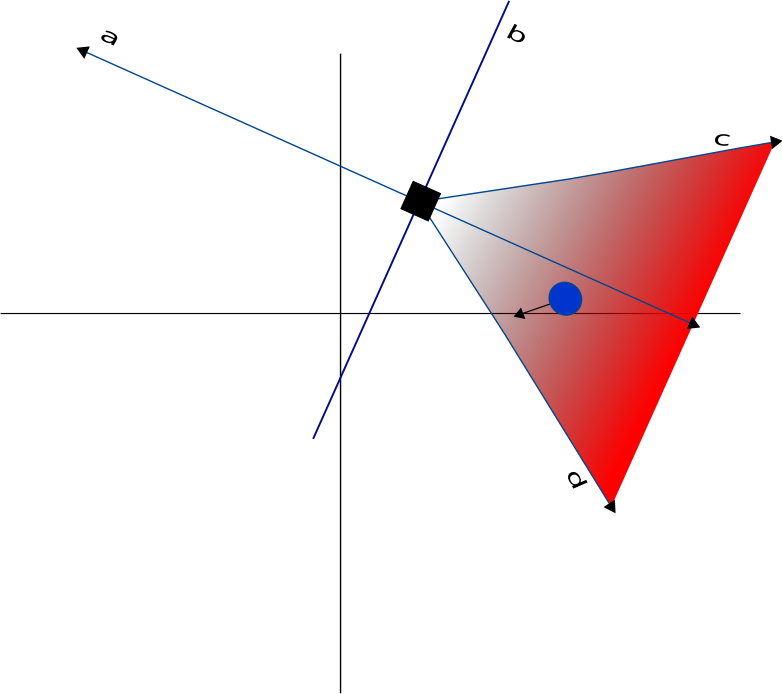
\includegraphics[width=175pt, height=175pt]{img/sweepal_start.png}
    }
    \hspace*{15pt}
    \subfigure[Translated system]{
      \label{fig:sweepal_translate}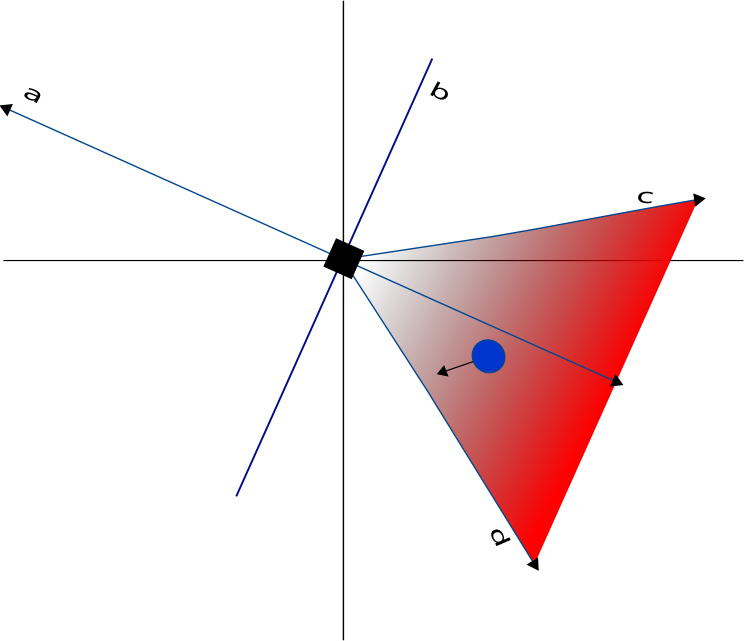
\includegraphics[width=175pt, height=175pt]{img/sweepal_translate.png}
    }

    \subfigure[Rotated system]{
      \label{fig:sweepal_rotate}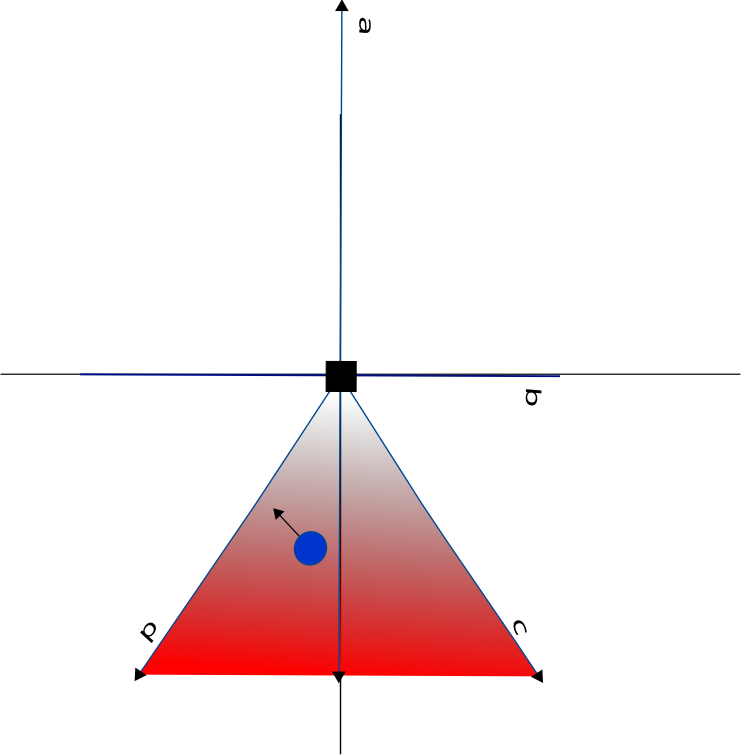
\includegraphics[width=175pt, height=175pt]{img/sweepal_rotate.png}
    } 
    \hspace*{15pt}
    \subfigure[Triangle AOB]{
      \label{fig:sweepal_triangle}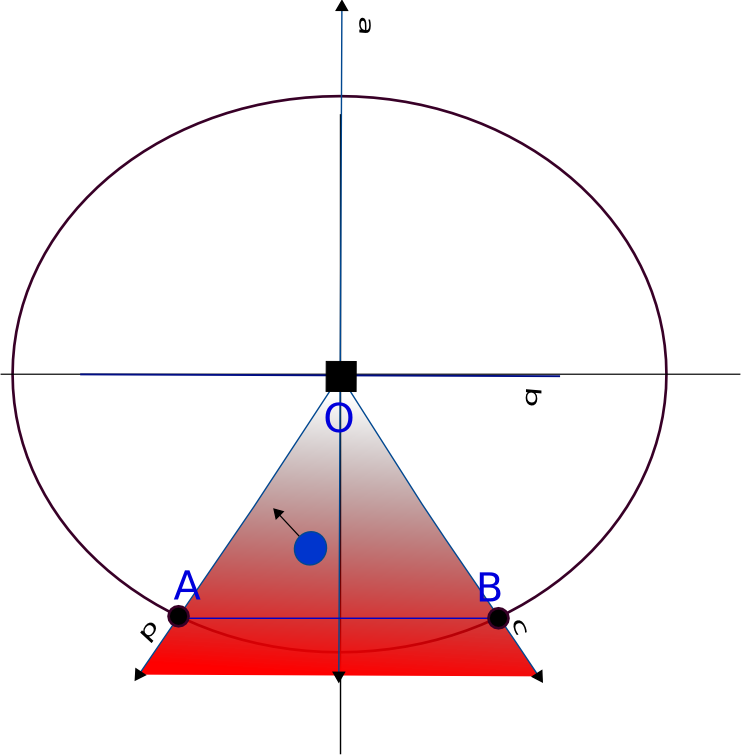
\includegraphics[width=175pt, height=175pt]{img/sweepal_triangle.png}
    } 

    \vspace*{20pt}
    \subfigure[Symbol definition]{
      \label{fig:sweepal_caption}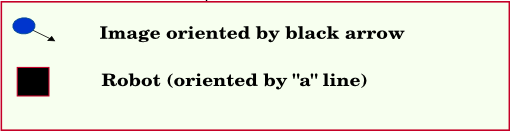
\includegraphics[width=255pt, height=65pt]{img/sweepal_caption.png}
    } 

  \end{center}
  \caption{WithinBoundaries algorithm}
  \label{fig:withingboundaries}
\end{figure}

%
Before checking whether a point (i.e. an image) is included 
whithin the \textit{sweep area}, the robot and image coordinates
are translated and then rotated, in order to move the robot in 
the origin of the axis and to overlap its orientation arrow with 
the y-axis. The two transformations are shown in figure 
\ref{fig:sweepal_translate} and \ref{fig:sweepal_rotate}, 
while the robot and image starting coordinates are shown in 
figure \ref{fig:sweepal_start}.
%

%
After executing these transformations, the sweep area is always 
situated in the second and third quadrant, as 
shown in figure \ref{fig:sweepal_rotate}. Now the "c" and "d" 
lines pass both from the origin.
%

%
If we draw a circle centered in the axis origin, the intersection 
between the circle and the "c" and "d" lines will
return four points in the plan. Among these, the points situated 
in the second and third quadrant define a triangle
with the centre of the XY axis: this will be our "sweep area", 
where to check if an image is included or not. Note
that we choose the points with negative Y value (named "A" and "B") 
due to the translation and rotation operated
before. Again, see figure \ref{fig:sweepal_triangle} 
for a graphical example.
%

%
The circle radius must be a value large enough to include a wide 
number of images. In our case we defined it with a
value of five hundred, in order to reduce the difference between 
the abstract "sweep area" and the actual triangle 
"AOB" (figure \ref{fig:sweepal_triangle}) used to simplify the algorithm.
%

%
We have now reduced the problem to check whether a point 
lies on the \textit{sweep area} to a well-known problem:
checking if a point is included whithin triangle
\cite{withinboundaries:pointintriangle}. 
%
The better (and more rapid) way to resolve such problem 
exploits the cross product between vectors
in three-dimensional Euclidean space.
%
\begin{figure}[!h]
  \begin{center}
    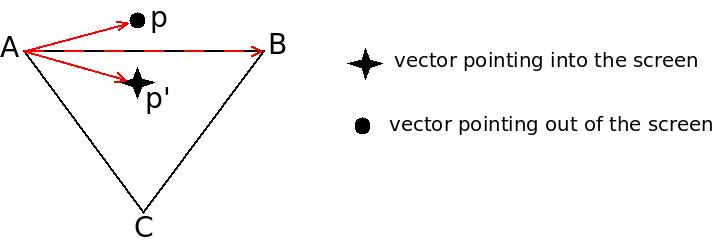
\includegraphics[width=300pt]{img/sweepal_crossproductABC.jpeg} 
    \caption{Cross product between vectors}
    \label{fig:sweepal_crossproductABC}
  \end{center}
\end{figure}
Referring to the image \ref{fig:sweepal_crossproductABC}, the cross product of [A-B] and [A-p] will result a vector
pointing out of the screen. On the other hand, the cross product of [A-B] and [A-p'] will result a vector pointing
into the screen.
%

%
The cross product of [A-B] with the vector from A to any point above the segment AB turns out with a resulting vector
points out of the screen, while using any point below AB yields with a vector pointing into the screen. We have to
distinguish which direction a resulting vector must have in order to consider the point "p" inside the triangle.
%

%
Because the triangle can be oriented in any way, what we need is a reference point, that is a point that we know is
on a certain side of the line. For our triangle (figure \ref{fig:sweepal_crossproductABC}), this is just the third
point C.
%

%
Any point "p", where [A-B] cross [A-p] does not point in the same direction as [A-B] cross [A-C], is not inside the
triangle. If the cross products do point in the same direction, then we need to test "p" with the other lines as well.
If the point was on the same side of AB segment as C, and is also on the same side of BC segment as A, and on the same
side of CA segment as B, then it is in the triangle.
%

%
The main disadvantage regarding the approach above described is that the sweep angle value must be strictly greater
than zero and strictly less than ninety degrees. If the sweep angle exceeds previous limits the algorithm will executes
with a wrong triangle AOB (we remember that AOB angle, shown in figure \ref{fig:sweepal_triangle}, is equal to twice
the sweep angle).
%
\subsubsection{The SweepMetricCalc class}
\label{subsubsec:sweep_metric_class}
Once we are done with the description of the algorithm, 
let us see how to actually use the \texttt{SweepMetricCalc} 
class. 
%

%
All is needed in order to use the class, is to instantiate it,
using its conversion constructor:
%
\begin{lstlisting}[caption={\texttt{SweepMetricCalc} class declaration}, label={code:sweepmetriccalc}, frame=trBL]
SweepMetricCalc::SweepMetricCalc( float sweep_angle,
				  float angle_offset,
				  float mu_distance,
				  float sigma_distance,
				  float mu_angle,
				  float sigma_angle );				  
\end{lstlisting}
%
Here is a brief description of the constructor parameters:
%
\begin{itemize}
  \item \texttt{sweep\_angle} \\
    half the angle which defines the \textit{sweep area}
  \item \texttt{angle\_offset} \\
    maximum difference allowed between robot and 
    image orientation 
  \item \texttt{mu\_distance} \\
    expected value (i.e. mean value) for the Gaussian 
    which assigns the score on the basis of distance between
    image and robot
  \item \texttt{sigma\_distance} \\
    standard deviation for the Gaussian which assigns the 
    score on the basis of distance between image and robot
  \item \texttt{mu\_angle} \\
    expected value (i.e. mean value) for the Gaussian which 
    assigns the score on the basis of orientation difference
    between image and robot
  \item \texttt{sigma\_angle} \\
    standard deviation for the Gaussian which assigns the 
    score on the basis of orientation difference between image
    and robot
\end{itemize}
%
